\begin{figure}
	\centering
	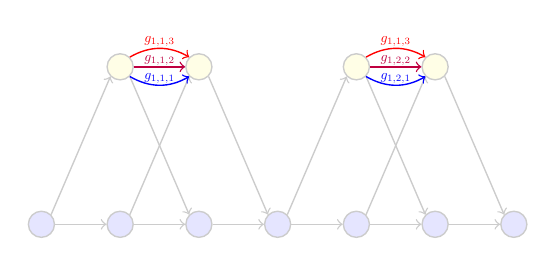
\begin{tikzpicture}[->, line width=0.5pt]
		\node[circle, fill=blue!10, draw=black!20,line width=0.5pt, minimum size=0.1in](one) at (0,0){};
		\node[circle, fill=blue!10, draw=black!20,line width=0.5pt, minimum size=0.1in](two) at (1,0){}; 
		\node[circle, fill=blue!10, draw=black!20,line width=0.5pt, minimum size=0.1in](three) at (2,0){};
		\node[circle, fill=blue!10, draw=black!20,line width=0.5pt, minimum size=0.1in](four) at (3,0){};
		\node[circle, fill=blue!10, draw=black!20,line width=0.5pt, minimum size=0.1in](five) at (4,0){};
		\node[circle, fill=blue!10, draw=black!20,line width=0.5pt, minimum size=0.1in](six) at (5,0){};
		\node[circle, fill=blue!10, draw=black!20,line width=0.5pt, minimum size=0.1in](seven) at (6,0){};
		\node[circle, fill=yellow!10, draw=black!20,line width=0.5pt, minimum size=0.1in](eight) at (1,2){};
		\node[circle, fill=yellow!10, draw=black!20,line width=0.5pt, minimum size=0.1in](nine) at (2,2){};
		\node[circle, fill=yellow!10, draw=black!20,line width=0.5pt, minimum size=0.1in](ten) at (4,2){}; 
		\node[circle, fill=yellow!10, draw=black!20,line width=0.5pt, minimum size=0.1in](eleven) at (5,2){}; 
		\draw [line width=0.5pt,color=black!20] (one.east) -- (two.west);
		\draw [line width=0.5pt,color=black!20] (two.east) -- (three.west);
		\draw [line width=0.5pt,color=black!20] (three.east) -- (four.west);
		\draw [line width=0.5pt,color=black!20] (four.east) -- (five.west);
		\draw [line width=0.5pt,color=black!20] (five.east) -- (six.west);
		\draw [line width=0.5pt,color=black!20] (six.east) -- (seven.west);
		\draw [line width=0.5pt,color=black!20] (one.north east) -- (eight.south west);
		\draw [line width=0.5pt,color=black!20] (two.north east) -- (nine.south west);
		\draw [line width=0.5pt,color=black!20] (four.north east) -- (ten.south west);
		\draw [line width=0.5pt,color=black!20] (five.north east) -- (eleven.south west);
		\draw [line width=0.5pt,color=black!20] (eight.south east) -- (three.north west);
		\draw [line width=0.5pt,color=black!20] (nine.south east) -- (four.north west);
		\draw [line width=0.5pt,color=black!20] (ten.south east) -- (six.north west);
		\draw [line width=0.5pt,color=black!20] (eleven.south east) -- (seven.north west);

		\draw [color=red,-,line width=0.5pt] (eight.north east) edge[->,bend left]node[above=-3pt]{\scalebox{0.5}{$g_{1,1,3}$}}(nine.north west);
		\draw [color=purple,line width=0.5pt] (eight.east) -- node[above=-3pt]{\scalebox{0.5}{$g_{1,1,2}$}}(nine.west);
		\draw [color=blue,-,line width=0.5pt] (eight.south east) edge[->, bend right]node[above=-3pt]{\scalebox{0.5}{$g_{1,1,1}$}}(nine.south west);

		\draw [color=red,-, line width=0.5pt] (ten.north east) edge[->, bend left]node[above=-3pt]{\scalebox{0.5}{$g_{1,1,3}$}}(eleven.north west);
		\draw [color=purple,line width=0.5pt] (ten.east) -- node[above=-3pt]{\scalebox{0.5}{$g_{1,2,2}$}}(eleven.west); 
		\draw [color=blue,-, line width=0.5pt] (ten.south east) edge[->, bend right]node[above=-3pt]{\scalebox{0.5}{$g_{1,2,1}$}}(eleven.south west);
	\end{tikzpicture}
	\caption{Multi-Rate Charging}
	\label{fig:multirateChargeEdges}
\end{figure} 
